\documentclass{beamer}

%% Configuración de la presentación
\mode<presentation> {

  \usetheme{Warsaw}

  
  \usecolortheme{beaver}
 
}

%% Fuentes de tamaño arbitrario
\usepackage{lmodern}
\usepackage{amsfonts}
\usepackage{dsfont}

%% Gráficos
\usepackage{graphicx} % Allows including images
\usepackage{booktabs} % Allows the use of \toprule, \midrule and \bottomrule in tables

%%% Castellano.
% noquoting: Permite uso de comillas no españolas.
% lcroman: Permite la enumeración con numerales romanos en minúscula.
% fontenc: Usa la fuente completa para que pueda copiarse correctamente del pdf.
\usepackage[english,spanish,es-noquoting,es-lcroman]{babel}
\usepackage[utf8]{inputenc}
\usepackage[T1]{fontenc}
\selectlanguage{spanish}

\usepackage{tikz}
\usepackage{tikz-cd}
\usepackage{tikz-3dplot}

\usepackage{verbatim}
\usetikzlibrary{arrows,shapes}
\usepackage{amsthm}
\usepackage{accents}
\usepackage{amsmath,amssymb,lmodern}

% Definitions
\theoremstyle{plain}
\newtheorem{thm}{Teorema}
\theoremstyle{definition}
\newtheorem{defn}[thm]{Definici\'{o}n}
\theoremstyle{plain}
\newtheorem{prop}[thm]{Proposici\'{o}n}
\theoremstyle{definition}
\theoremstyle{remark}
\newtheorem{rem}[thm]{Nota}
\theoremstyle{definition}
\newtheorem{lem}[thm]{Lema}
\newtheorem{cor}[thm]{Corolario}
\newtheorem{ejemplo}[thm]{Ejemplo}
\newtheorem{ejemplos}[thm]{Ejemplos}
% Counter

\newcounter{saveenumi}
\newcommand{\seti}{\setcounter{saveenumi}{\value{enumi}}}
\newcommand{\conti}{\setcounter{enumi}{\value{saveenumi}}}

% Sections
\AtBeginSection{\frame{\sectionpage}}
\newtranslation[to=spanish]{Section}{Sección}

%comandos para agilizar la escritura de simbolos frecuentes
\newcommand{\sphere}{\mathds{S}^{d-1}}
\newcommand{\esfera}{\mathds{S}^{2}}
\newcommand{\orto}{\mathbb{O}^d}
\newcommand{\R}{\mathds{R}^d}
\newcommand{\spharm}{\mathds{Y}^d_n}
\newcommand{\sphint}{\int_{\sphere}}

\defbeamertemplate{section page}{mine}[1][]{%
  \begin{centering}
    {\usebeamerfont{section name}\usebeamercolor[fg]{section name}#1}
    \vskip1em\par
    \begin{beamercolorbox}[sep=12pt,center]{part title}
      \usebeamerfont{section title}\insertsection\par
    \end{beamercolorbox}
  \end{centering}
}

%----------------------------------------------------------------------------------------
%	TÍTULO
%----------------------------------------------------------------------------------------

\title[Distribución de puntos en la esfera.Competición en Kaggle.]{Distribución de puntos en la esfera.\\ Competición en Kaggle.} % The short title appears at the bottom of every slide, the full title is only on the title page

\author{Daniel López García} % Your name
\institute[UGR] % Your institution as it will appear on the bottom of every slide, may be shorthand to save space
{
  Universidad de Granada \\ % Your institution for the title page
  % Your email address
}
\date{26 de junio de 2018} % Date, can be changed to a custom date



\begin{document}
% Spanish
\selectlanguage{spanish}
% Para tikz
\pgfdeclarelayer{background}\theoremstyle{definition}
\pgfsetlayers{background,main}
% Secciones
\setbeamertemplate{section page}[mine]

%% Diapositiva de título.
\frame{\titlepage}

%% Diapositiva de contenidos.
% Throughout your presentation, if you choose to use \section{} and \subsection{} commands,
% these will automatically be printed on this slide as an overview of your presentation
\begin{frame}
  \frametitle{Contenidos} % Table of contents slide, comment this block out to remove it
  \tableofcontents
\end{frame}


%----------------------------------------------------------------------------------------
%	PRESENTACIÓN
%----------------------------------------------------------------------------------------

%------------------------------------------------
\section{Distribución de puntos en la esfera.} % Sections can be created in order to organize your presentation into discrete blocks, all sections and subsections are automatically printed in the table of contents as an overview of the talk
%------------------------------------------------
\begin{frame}
	
	\frametitle{Objetivos}
	\begin{itemize}
		\item Determinar conjuntos de puntos
		para aproximación, interpolación e integración sobre la esfera y sus propiedades geométricas.
		\item Simulación y visualización de distribuciones de puntos sobre la esfera.
	\end{itemize}
	
\end{frame}

\subsection{Armónicos Esféricos.}
\begin{frame}
	\tableofcontents[currentsection,currentsubsection,sections=1]
\end{frame}
\begin{frame}
	\frametitle{Espacios de Polinomios Homogéneos.}
	Consideramos $\mathcal{H}^d_n$ el espacio de polinomios homogéneos de grado n en d dimensiones.
	Estas funciones son de la forma:
	\begin{gather*}
		\sum_{|\alpha|=n}a_\alpha x^\alpha, a_\alpha \in \mathds{C}
	\end{gather*}

	\begin{ejemplos}
		\begin{gather*}
		\begin{aligned}
		\mathcal{H}^2_2 &= \{ a_1x_1^2 + a_2x_1x_2 + a_3x_2^2\} \\
		\mathcal{H}^2_3 &= \{ a_1x_1^3 + a_2x_2^3 + a_3x_1^2x_2 + a_4x_1x_2^2 \}
		\end{aligned}
		\end{gather*}
	\end{ejemplos}
\end{frame}

\begin{frame}
	\begin{defn}
		Una función f es armónica si $\triangle f (x) = 0$, es decir $$\frac{\partial^2 f}{\partial x_1^2}+\frac{\partial^2 f}{\partial x_2^2}+...+\frac{\partial^2 f}{\partial x_n^2} = 0$$
	\end{defn}

	Llamamos $\mathds{Y}_n(\mathds{R}^d)$ al espacio de los polinomios homogéneos de grado n en $\mathds{R}^d$ que son armónicos.

\end{frame}
\begin{frame}
	\frametitle{Armónicos Esféricos.}
	\begin{defn}
		Se llama espacio de armónicos esféricos de orden $n$ en $d$ dimensiones a	$\mathds{Y}^d_n = \mathds{Y}_n(\mathds{R}^d)_{|\mathds{S}^{d-1}}$ 
	\end{defn}
	De la definición se deduce que un armónico esférico $\mathds{Y}_n \in \mathds{Y}^d_n$ está asociado a un armónico homogéneo $\mathds{H}_n \in \mathds{Y}_n$ de la siguiente forma:
	$$
	\mathds{H}_n(r\xi) = r^n\mathds{Y}_n(\xi)
	$$
\end{frame}
\begin{frame}
	\frametitle{Base ortogonal}
	\begin{thm}
		Sean, $T_{n}(t),U_{n}(t)$ los polinomios de Chebyshev de 1ª y 2ª clase respectivamente.Y definimos
		\begin{gather*}
		g_{0,n}(x_1,x_2) = (x_1^2+x_2^2)T_n^2(x_2(x_1^2+x_2^2)^{-1/2})
		\\
		g_{1,n-1}(x_1,x_2) = x_1(x_1^2+x_2^2)^{\frac{n-1}{2}}U_{n-1}(x_2(x_1^2+x_2^2)^{-1/2})
		\end{gather*}
		entonces, si tomamos $\textbf{n}=(n_1,...,n_d)$ con $n_1 = \{0,1\}$ se define
		\begin{gather*}
		Y_{\textbf{n}}=g_{n_1,n_2}(x_1,x_2)\prod_{j=3}^{d}(x_1^2+...+x_j^2)^{n_j/2}C_{n_j,\lambda_j}(x_j(x_1^2+...+x_j^2)^{-1/2})
		\end{gather*}
		donde $\lambda_j =\lambda_j(n_1,...,n_{j-1}) = \sum_{i=1}^{j-1}n_i + \frac{j-2}{2}$. Entonces $\{Y_n,|\textbf{n}|=n\}$ es una base de $\mathds{Y}_{n}^{d}$.
	\end{thm}
\end{frame}
\subsection{Cálculo del gradiente.}
\begin{frame}
	\tableofcontents[currentsection,currentsubsection,sections=1]
\end{frame}

\begin{frame}
		\frametitle{Caso particular. Esfera de dimensión 3.}
		Tomando coordenadas esféricas,
		\begin{gather*}
		\begin{aligned}
		x_1 &= r \sen \theta \sen \phi\\
		x_2 &= r \sen \theta \sen \phi\\
		x_3 &= r \cos \theta\\
		\end{aligned}
		\\
		0\le \theta \le \pi,0\le\phi\le2\pi,r>0
		\end{gather*}
		una base ortogonal de $\mathds{Y}_n^3$ viene dada por
		\begin{equation*}
		\left\lbrace
		\begin{array}{ll}
		Y^n_ {k,1} = (\sen \theta)^kC_{n-k,k+1/2}(\cos \theta) \cos(k\phi),\quad 0\le k\le n \\
		Y^n_{k,2}(x) = (\sen\theta)^kC_{n-k,k+1/2}(\cos\theta)\sen(k\phi), \quad 1\le k\le n
		\end{array}
		\right.
		\end{equation*}
\end{frame}
\begin{frame}
La expresión de las parciales es la siguiente:
	\begin{prop} Para $k=0,...,n$
		\begin{gather*} 
		\begin{aligned}
		\partial_1Y^{n}_{k,1}(x) &= -\frac{(n+k)(n+k-1)}{2(2k-1)}Y^{n-1}_{k-1,2}(x)-(k+\frac{1}{2})Y^{n-1}_ {k+1,2}(x) \\
		\partial_2Y^{n}_{k,1}(x) &= \frac{(n+k)(n+k-1)}{2(2k-1)}Y^{n-1}_{k-1,1}(x)-(k+\frac{1}{2})Y^{n-1}_ {k+1,1}(x) \\
		\partial_3 Y_{k,1}^{n}(x) &=(n+k)Y_{k,1}^{n-1}(x)
		\end{aligned}
		\end{gather*}

	\end{prop}
\end{frame}
\begin{frame}
	\frametitle{Puntos críticos del gradiente.}

	Igualando las expresiones de las parciales a 0 tenemos que 
	\begin{gather*}
	\left\{
	\begin{array}{ll}
	\sen \theta= 0 \\
	\cos k\phi = 0 &\\
c_{n,k}C_{n-k}^{k-1/2}(cos \theta) + d_k sen^2\theta C_{n-k-2}^{k+3/2}(cos \theta) = 0
	\end{array}
	\right.
	\end{gather*}
	De estas condiciones se deduce que existen, $2k(n-k)+2$ puntos que anulan el gradiente.
\end{frame}

\subsection{Integración numérica.}
\begin{frame}
	\tableofcontents[currentsection,currentsubsection,sections=1]
\end{frame}
\begin{frame}
	\frametitle{Integración de puntos dispersos.}
	Supongamos que tenemos N nodos, $P=\{\eta_1,...,\eta_N\}$ y sus valores aproximados $f_i~\approx f(\eta_i)$. Queremos aproximar la integral $$I(f) =  \int_{\mathds{S}^2} f(\eta)dS^2(\eta)$$.
	\begin{prop}
		Sea $T_N=\{\triangle_1,...,\triangle_{M(N)}\}$ la triangulación de $\mathds{S}^2$, donde los vértices de cada triángulo son los nodos.
		\begin{gather*}
		\begin{aligned}
			I(f) &= \sum_{k=1}^{M} \int_{\triangle_k} f(n)dS^2(n) \\& \approx  \sum_{k=1}^{M} \frac{1}{3}[f(n_{k,1})+f(n_{k,2})+f(n_{k,3})] area(\triangle_k)
		\end{aligned}
		\end{gather*}
	\end{prop}
\end{frame}
\begin{frame}
		\frametitle{Integración de puntos dispersos.}
		\begin{prop}
			$|I(f)-I_n(f)|\le 4\pi c_f \max$ diam$(\triangle) \quad \triangle\in T_N$
		\end{prop}
	La bondad de la aproximación depende de la triangulación y del conjunto de nodos elegidos.
	Es conocido que se obtienen buenos resultados tomando un conjunto en el que los puntos están bien distribuidos.

\end{frame}
\section{Competición en Kaggle.}

\subsection{Introducción.}
\begin{frame}
	\tableofcontents[currentsection,currentsubsection,sections=2]
\end{frame}
\begin{frame}
	\frametitle{Descripción del problema.}
	Queremos detectar cuando se registran clicks en los anuncios y estos no conllevan la instalación de la app a partir de los siguientes datos.
\begin{itemize}
	
	\item ip: dirección IP de click.
	\item app: id de la aplicación
	\item device: identificación del tipo de dispositivo del teléfono móvil del usuario
	\item channel: id del canal del editor publicitario móvil
	\item so: id de la versión del OS del teléfono móvil del usuario
	\item click\_time: marca de tiempo del click 
	\item attributed\_time : momento de la descarga de la aplicación 
	\item is\_attributed : el objetivo que se va a pronosticar, indica si la aplicación se descargó
\end{itemize}
\end{frame}
\subsection{Preprocesamiento}
\begin{frame}
	\tableofcontents[currentsection,currentsubsection,sections=2]
\end{frame}
\begin{frame}
	\frametitle{Visualización de los datos.}
	Para poder elegir una estrategia para el preprocesamiento es necesario
	realizar una visualización de los datos.De esta forma, podremos obtener
	cómo están distribuidos los valores de cada uno de los atributos o si existe alguna relación de correlación entre ellos.
	\medskip
	
	Tras realizar el estudio de los datos se obtienen las siguientes conclusiones:
		\begin{itemize}
		\item La columna $attributed\_time$ puede ser eliminada ya que la mayoría de sus valores son vacíos.
		\item De la variable $click\_time$ podemos obviar los datos relativos al mes y al año.
		\item Las variables $os$ y $device$ representan la misma información.
		\item Existe un gran desbalanceo de clases.
	\end{itemize}
\end{frame}
\begin{frame}


	\begin{columns}[t]
		\column{.5\textwidth}
		\centering
	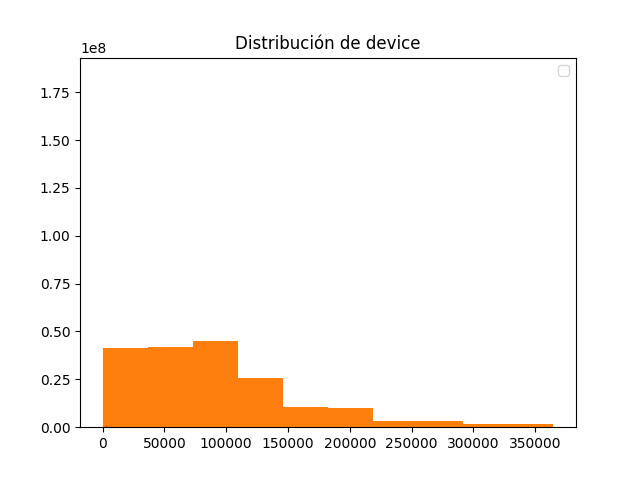
\includegraphics[scale=0.4]{../img/device_distribution.png}\\

	
		\centering

	\column{.5\textwidth}
				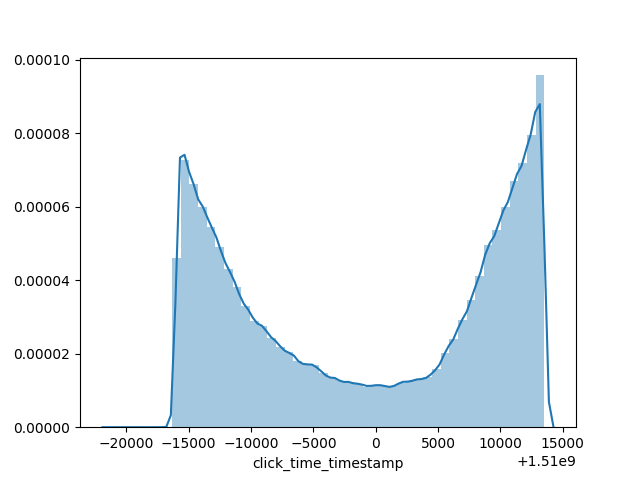
\includegraphics[scale=0.4]{../img/normalDistclick_time_timestamp.png}
	\end{columns}
\end{frame}
\begin{frame}
		\begin{columns}[t]
		\column{.5\textwidth}
		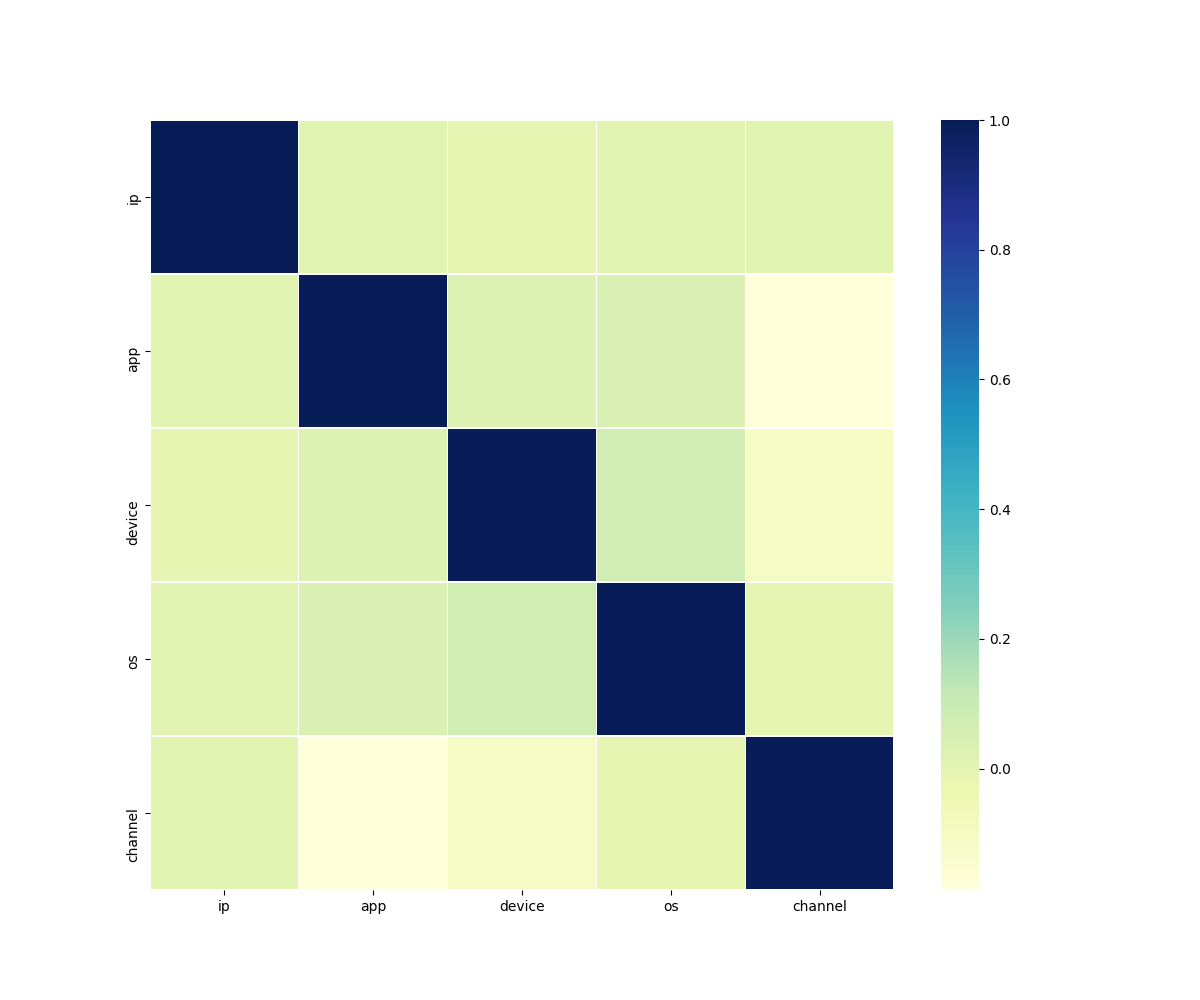
\includegraphics[scale=0.25]{../img/correlation.png}
		\column{.5\textwidth}
	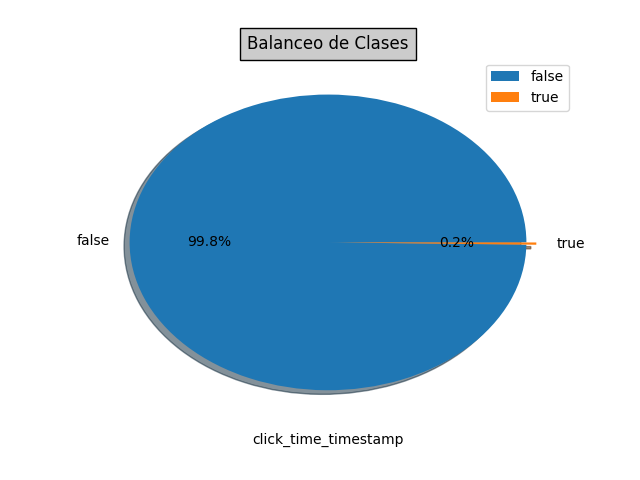
\includegraphics[scale=0.35]{../img/imbalacing.png}
		\end{columns}
	\end{frame}
\begin{frame}
	\begin{table}[H]
		\centering
		\begin{tabular}{lllll}
			Atributo& Total & \%    \\
			ip	& 0 &0 \\
			app	& 0 & 0   \\
			os	& 0 & 0 \\
			chanel &0 & 0 \\
			device & 0 & 0  \\
			click\_time& 0& 0 \\
			attributed\_time &184447044& 99.7529
		\end{tabular}
		\caption{Valores perdidos.}
		\label{}
	\end{table}
	\end{frame}
\begin{frame}
	\frametitle{Preprocesamiento.}
	\begin{enumerate}
		\item Eliminar la columna attributed\_time,
			\item Obtener los datos timestamp y día de la variable click\_time.
		\item Agrupar las variables categóricas.
		\begin{itemize}
			\item Teniendo en cuenta el número de apariciones.
			\item Usando el valor medio.
		\end{itemize}
\end{enumerate}
\end{frame}

\begin{frame}
	La siguiente tabla recoge los resultados obtenidos en las distintas fases del preprocesamiento.
	\begin{table}[H]
		\centering
		
		\begin{tabular}{ll}
			\textbf{Cambio realizado}& \textbf{Resultado} \\
			\hline
			\\
			Conjunto inicial& 0.8385028     \\
			Eliminar mes,año y click\_time& 0.8471159  \\
			Añadir día y hora&  0.8471159 \\
			Cambiar día por día de la semana & 0.8471159\\
			count(channel) tras agrupar ip-app e ip-app-os & 0.8289424 \\
			count(channel) tras agrupar ip-day e ip-day-hour & 0.8569927 \\
			media(channel) tras agrupar ip-app e ip-app-os & 0.8559159 \\
			media(channel) tras agrupar ip-day e ip-day-hour & 0.8628768 \\
			Conjunto final & 0.8649459
		\end{tabular}
		\caption{Pruebas realizadas durante el preprocesamiento.}
	\end{table}
\end{frame}
\subsection{Algoritmos usados.}
\begin{frame}
	\tableofcontents[currentsection,currentsubsection,sections=2]
\end{frame}
	\begin{frame}
		\frametitle{Algoritmos Usados.}
		Los algoritmos elegidos para construir un clasificador han sido los siguientes:
	\begin{itemize}
		\item Como punto de partida usaremos el algoritmo Boosting.
			\begin{itemize}
				\item Se han estudiado los parámetros que lo componen y se han optimizado algunos de ellos.
				\item Se ha balanceado el conjuntos de datos de entrenamiento.
			\end{itemize} 
		\item Se han estudiado algunas variantes como RUSBoosting y CUSBoosting.
	\end{itemize}
	\end{frame}
\begin{frame}
	La siguiente tabla recoge los resultados obtenidos.
	\begin{table}[H]
		\centering
		\begin{tabular}{ll}
			\textbf{Algoritmo}& \textbf{Resultado} \\
			\hline
			\\
			Boosting base&    0.9509598  \\
			Boosting con parámetros optimizados& 0.9769301 \\
			RUSBoosting & 0.8763027 \\
			CUSBoosting &  -  \\
			Boosting con conjunto balanceado & 0.9441415  \\
		\end{tabular}
		\caption{Resultados obtenidos con los diferentes algoritmos.}
	\end{table}
\end{frame}
\subsection{Resultados obtenidos.}
\begin{frame}
	\tableofcontents[currentsection,currentsubsection,sections=2]
\end{frame}
\begin{frame}
	\frametitle{Resultados obtenidos.}
	\begin{itemize}
		\item Los resultados obtenidos en esta última sección no han sido tan satisfactorios como a priori esperaba, ya que la aplicación de algoritmos alternativos no ha mejorado los resultados.
		\item Tras obtener los mejores parámetros del algoritmo Boosting hemos mejorado la puntuación un 2,73\%.
		\item Durante la fase de preprocesamiento hemos mejorado el rendimiento de nuestro clasificador un 3 \% aproximadamente.
	   
	\end{itemize}
\end{frame}
\end{document}
